\documentclass{ctexart}
\usepackage[a4paper,top=3cm,bottom=2.7cm,left=2.54cm,right=2.54cm]{geometry}
\usepackage{amsmath,amsfonts,amssymb,amsthm}
\usepackage{graphics}
\usepackage{tikz}
\usepackage{multirow}
\usepackage{array}
\usepackage{fancyhdr}
\usepackage{lastpage}
\usepackage{indentfirst}
\usepackage{draftwatermark}         % 所有页加水印
%\usepackage[firstpage]{draftwatermark} % 只有第一页加水印
\SetWatermarkText{半导体物理-期中-模拟}           % 设置水印内容
%\SetWatermarkText{\includegraphics{fig/texlion.png}}         % 设置水印logo
\SetWatermarkLightness{0.8}             % 设置水印透明度 0-1
\SetWatermarkScale{0.3}   
\pagestyle{fancy}
\fancyhf{}
\cfoot{第 \thepage 页 \quad 共 4 页}
\rhead{2024—2025 学年第一学期\quad }
\lhead{命题:Z\qquad 验题:M}
\renewcommand{\headrulewidth}{0.7pt}
%\renewcommand{\labelenumi}{\Arabic{enumi}}

\begin{document}

\vspace{1em}
\begin{center}

\textbf{\LARGE NJUIC 《 半导体物理学 》期中模拟考试试卷}
\end{center}

\begin{center}
\begin{tabular}{m{0.3\textwidth} m{0.3\textwidth} m{0.3\textwidth}}
     
     考试时长:120分钟 & 考生学号:&考生姓名:
\end{tabular}
\end{center}
\vspace{-0.3cm}
\hrule height 0.5pt
%\noindent
%\rule{\textwidth}{1pt}

\subsection*{一、(30 分)简答}

1. 什么是晶体点阵?和晶体结构的关系是什么?原胞取法唯一吗?\par
2. 晶体的晶面是什么?密勒指数是什么(仅考虑立方晶系),该如何确定? \par
3. 倒空间如何理解?正空间WS原胞与倒空间的第一布里渊区分别是如何选取的?\par
4. 能带理论中,周期场近似是什么?紧束缚近似是什么?布洛赫波函数是怎样的?\par
5. 如何理解电子共有化运动?能带是连续的吗?\par
6. 如何定义有效质量?其意义是什么?什么是间接带隙半导体?\par
7. 晶体的本征缺陷有哪些?掺杂为什么能够改变半导体导电性能?\par
*. 你如何理解什么是半导体?\par
\newpage

\subsection*{二、(10分)}

晶体结构的确定对了解晶体的性质非常重要,X射线衍射是确定晶体结构的重要手段.\par
1. 常见的铝晶体是一种面心立方堆积结构,Z同学用$\lambda_1 =1.54 \times 10 ^{-10}$m 的X射线做衍射分析,结果得到(110)面的衍射角$\theta_1$约为$22.3^{\circ}$.请给出晶体中一个铝原子的最近邻原子数,并分析上述结果的合理性.\par
2. Z同学又使用波长$\lambda_2 = 0.071$nm 的射线对一铁晶体做衍射分析,发现随着衍射角从零开始增大,最早在$\theta_2 = 10.1^{\circ}$ 时出现衍射峰.查阅资料知常温下铁晶体结构如下,晶格常数为$2.87\mathring{\text{A}}$.请给出该衍射峰对应晶面的晶面指数,并计算铁晶体原胞的体积.
\vspace{-0.2cm}
\begin{figure}[htbp]
    \flushright
    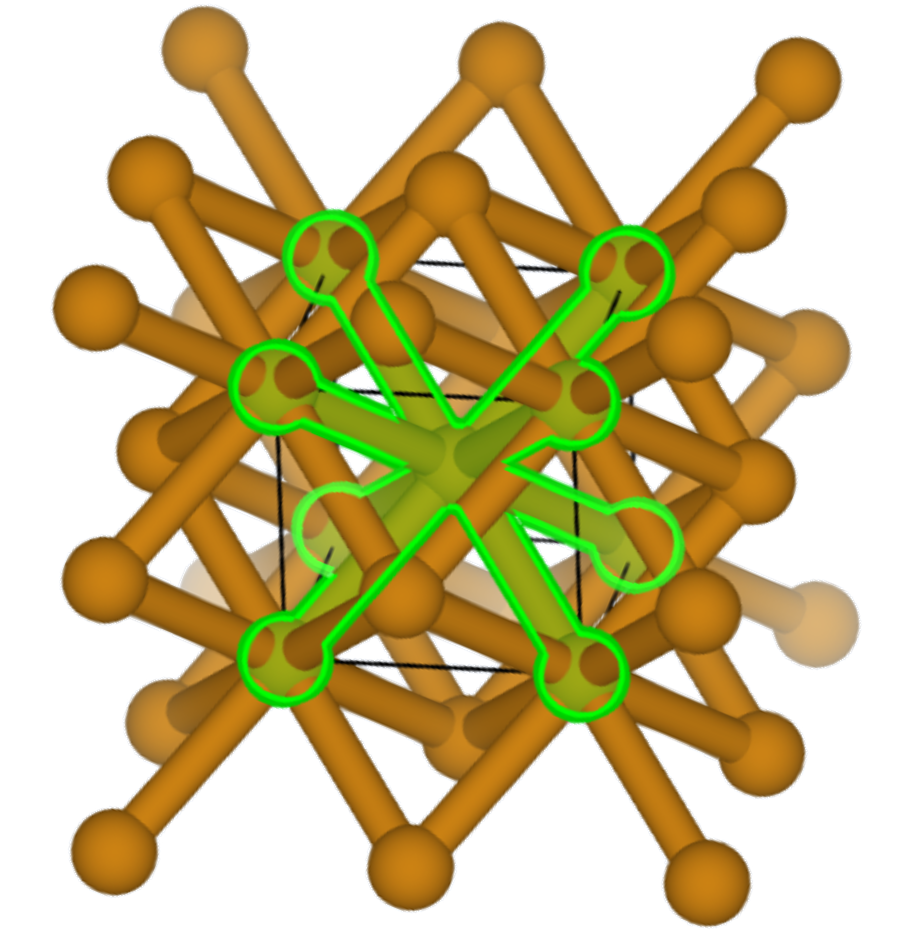
\includegraphics[width=0.23\textwidth]{1.png}
\end{figure}

\vspace{2cm}

\subsection*{三、(12分)}

与原子核的分裂与结合一样,晶体的形成常常伴随着能量的释放.考虑一个由两种二价离子(各$N$个,$N\rightarrow +\infty$)等间距组成的一维晶体,相互作用能为
\[
U(r)=-\frac{1}{2}\cdot 2N\Biggl[\frac{z_{1}z_{2}e^{2}}{4\pi\varepsilon_{0}r}\sum_{i(\neq j)}^{2N}(\pm\frac{1}{a_{i}})-\frac{B}{r^{n}}\Biggr]
\]

1. 请计算该晶体的Madelung常数$\alpha = \sum_{i(\neq j)}^{N}(\pm\frac{1}{a_{i}})$.\par
2. 若$n=4$,请计算单离子的结合能$E=u(r_0)$,可用平衡间距$r_0$表示.\par
3. 若$r_0=0.3$nm,结合能$E=3$ eV,试求$B$.

\newpage
\subsection*{四、(12 分)}

考虑室温300 K环境下一掺杂半导体硅,其$N_{\text{c}}=2.8\times 10^{19}$cm$^{-3}$,$E_\text{{g}} = 1.12$eV.\par
1. 半导体中首先掺杂了磷原子,使其费米能级来到导带底部下侧0.3 eV处,试计算磷的掺杂浓度并绘制能带图,体现出电离过程. 设杂质磷的电离能为0.04 eV.\par
2. 对上述硅继续掺杂硼原子,使得费米能级降低了0.1 eV,试计算硼的掺杂浓度. 假设均能全部电离.\par
3. 请简述下列各个能带图分别表明半导体处于何种掺杂情况,并分别指出哪个符合上述1、2小题的半导体掺杂情况.
\vspace{-0.3cm}
\begin{figure}[htbp]
    \flushright
    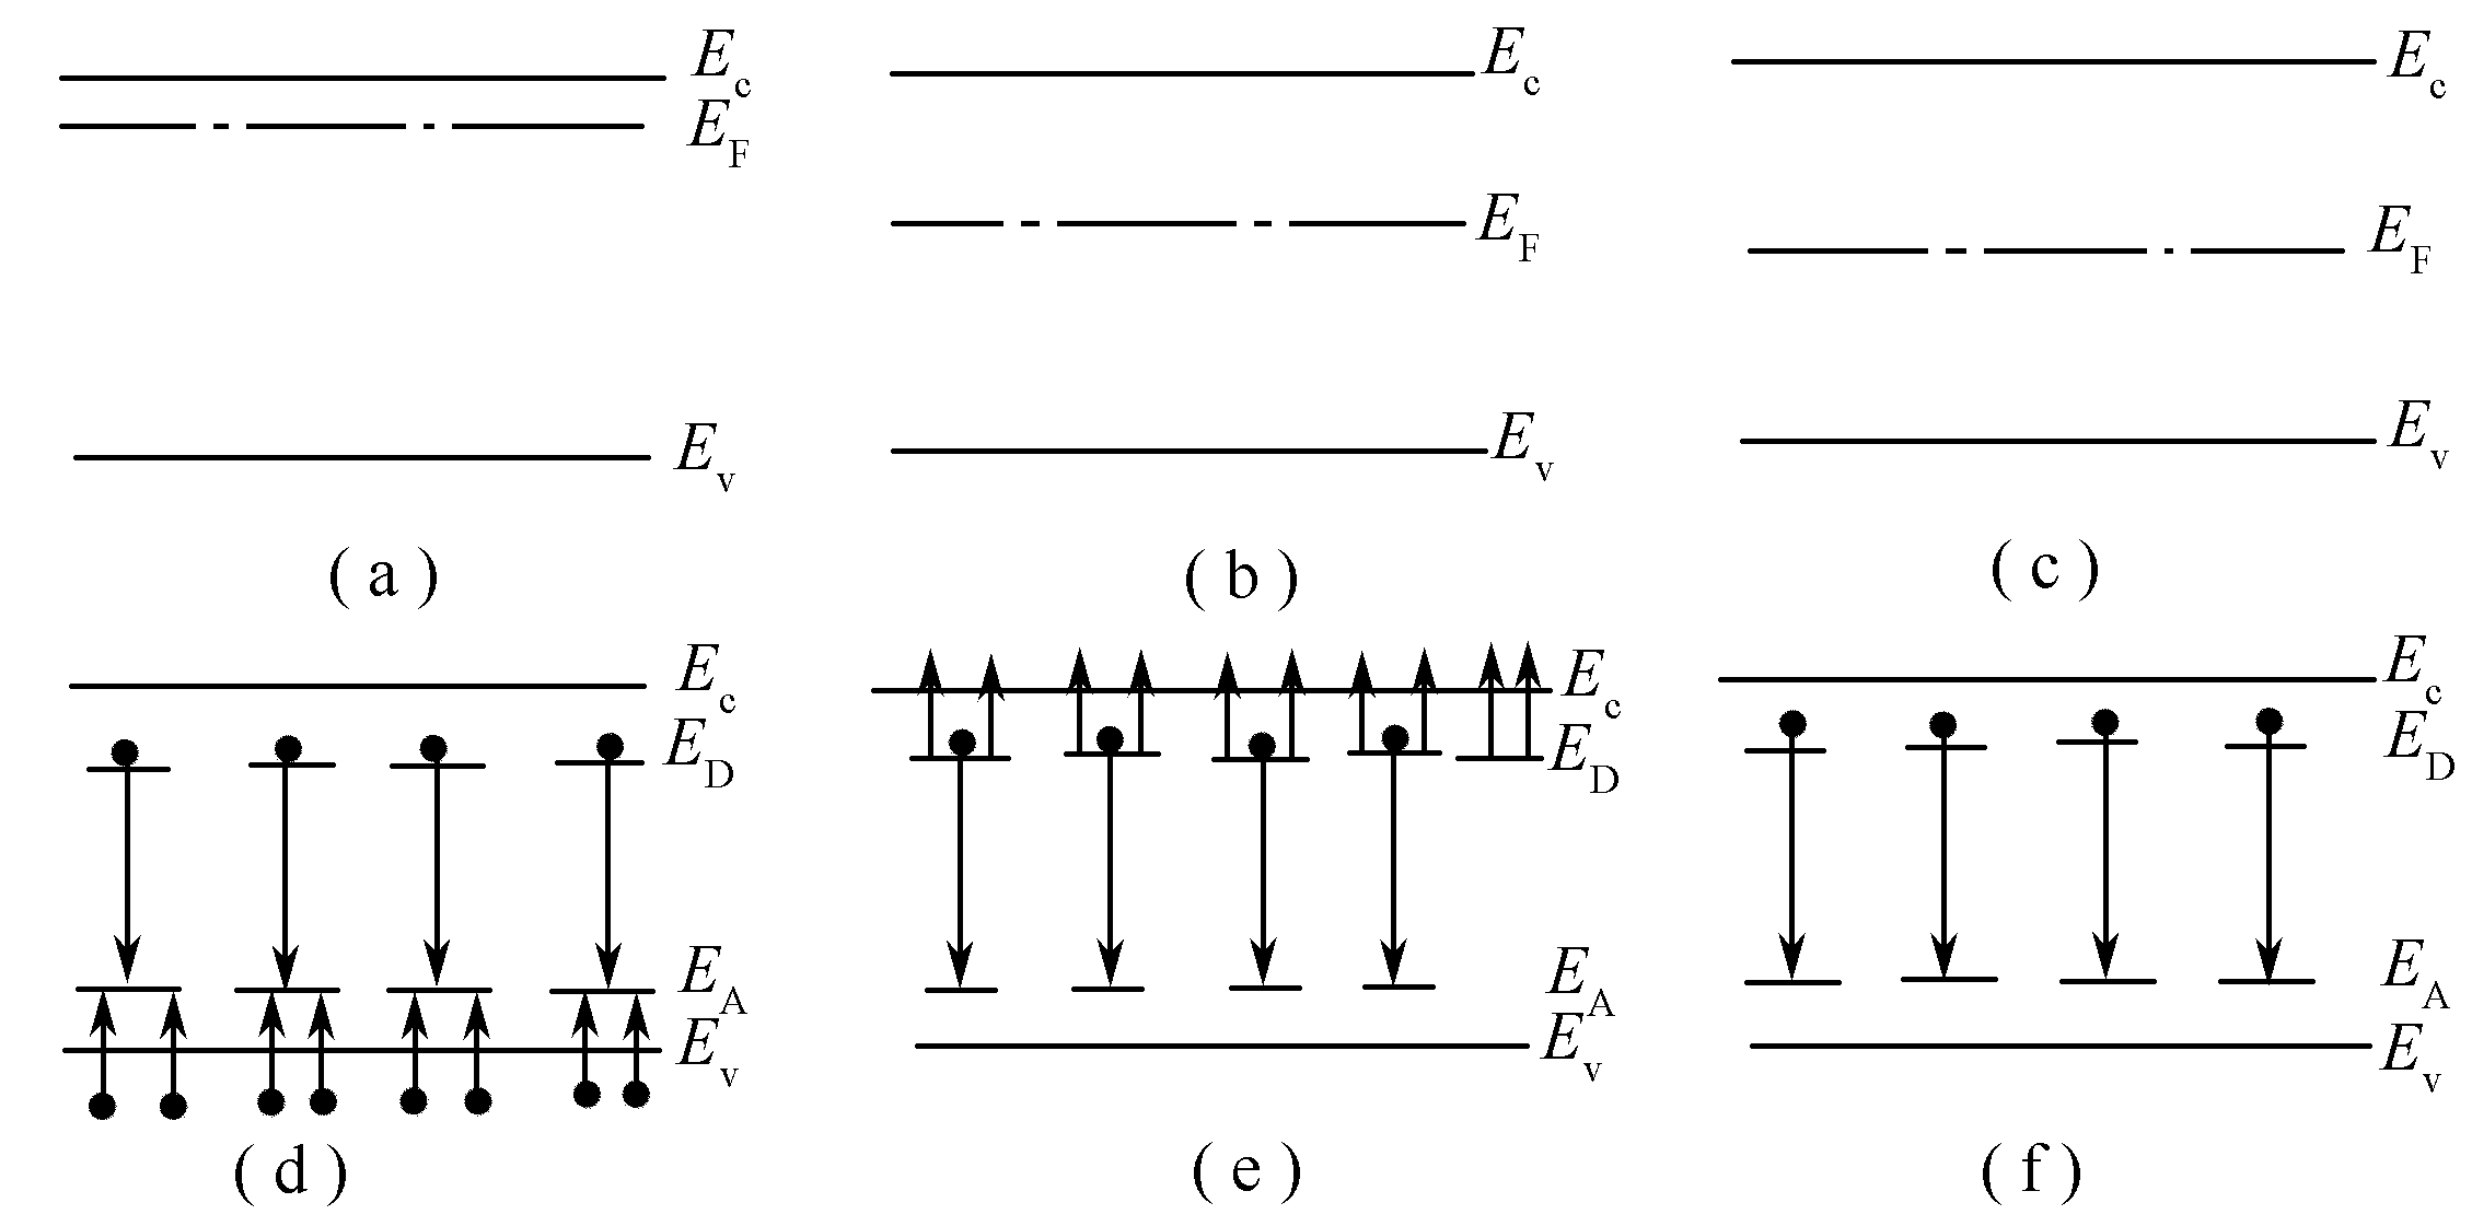
\includegraphics[width=0.65\textwidth]{2.png}
\end{figure}
\vspace{2.8cm}

\subsection*{五、(12 分)}
一块有杂质补偿的硅材料,已知掺入受主密度$N_\text{A} =1\times10^{15} \text{cm}^{-3}$,室温下测得其$E_\text{F}$恰好与$E_\text{D}$重合,并得知平衡电子密度为$n_0=5\times10^{15}\mathrm{cm}^{-3}$.已知室温下硅的本征载流子密度$1\times10^{10}\mathrm{cm}^{-3}$,导带底有效态密度$2.8\times10^{19}\text{cm}^{-3}$.\par
1. 请计算平衡少子浓度与$E_\text{F}$的位置.\par
2. 请计算掺入材料中的施主杂质浓度以及电离程度.\par
3. 导带底有效态密度$N_\text{c}\propto T^{\frac{3}{2}}$,请证明强电离条件下有$E_\text{F}=E_\text{c}+kT \ln \dfrac{N_\text{D} - N_\text{A}}{N_\text{c}}$,并简单说明该硅材料在$T=400$K 时的电离情况.

\newpage
\subsection*{六、(12 分)}
Z同学采购了两块硅材料,是杂质相同但浓度不同的两块n型硅.测量得到其电子浓度与温度的关系如图所示.试分析以下问题.\par
1. 两样品掺杂浓度较高的是哪个,在$T_A$左侧为什么两曲线近似重合.\par
2. 两曲线在$T_C$与$T_D$之间为什么近乎平行,为什么两平行曲线的起点$T_B$、$T_C$的不一致,终点$T_D$、$T_E$也不一致.\par
3. 若低温下,$N_{\text{c}}$近乎不变,则在$T_E$右侧两曲线是否平行,其斜率的含义是什么.\par
4. 请直接在图中绘制样品2的本征载流子浓度与温度的关系(纵坐标为$\ln n_{\text{i}}$).
\vspace{-0.2cm}
\begin{figure}[htbp]
    \flushright
    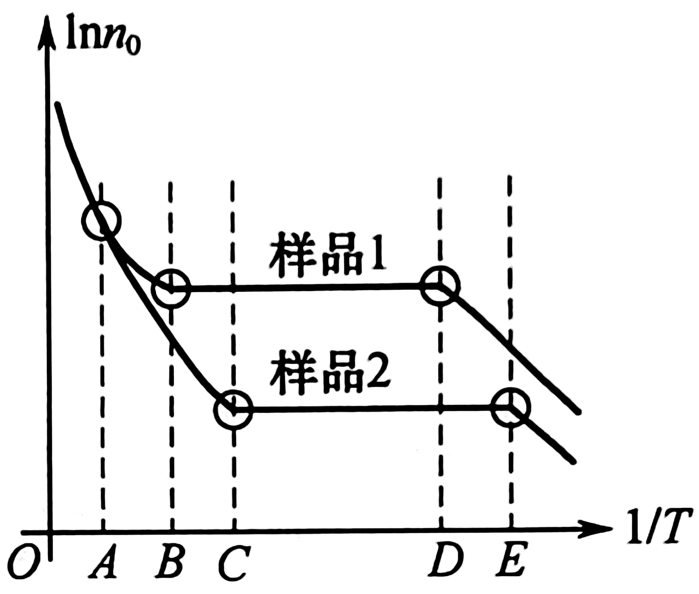
\includegraphics[width=0.4\linewidth]{3.png}
\end{figure}

\vspace{5cm}
\subsection*{七、(12 分)}
Z同学有一个n型锗样品,在300K环境下,其电子浓度$n_0=5\times10^{14}\text{cm}^{-3}$,试计算上述温度时掺杂锗的电导率$\sigma$.已知$\mu_\text{n}=3800 \text{cm}^2/(\text{V}·\text{s})$、$ \mu_\text{p}=1900 \text{cm}^2/(\text{V}·\text{s})$、$ n_\text{i}=2.33×10^{12}\text{cm}^{-3}$.


\end{document}
